\documentclass[a4paper,11pt]{article}
\usepackage[utf8]{inputenc}
\usepackage[T1]{fontenc}
\usepackage{amsmath,amssymb}
\usepackage[a4paper,left=2cm,right=2cm,top=3.6cm,bottom=2.3cm,headheight=1.1cm,headsep=0.6cm,footskip=1cm]{geometry}
\usepackage{xcolor}
\usepackage{tikz}
\usetikzlibrary{calc,arrows.meta,positioning,shapes.geometric,matrix}
\usepackage{fancyhdr}
\usepackage{lastpage}
\usepackage{tabularx}
\usepackage{array}
\usepackage[most]{tcolorbox}
\usepackage{enumitem}
\usepackage{needspace}

% ---------- palet sky (Sky-800 dan Sky-200) ----------
\definecolor{mainc}{HTML}{075985}
\definecolor{accc}{HTML}{0284C7}
\definecolor{skyl}{HTML}{BAE6FD}
\definecolor{deepc}{HTML}{082F49}
\definecolor{softbg}{HTML}{F0F9FF}
\definecolor{warmc}{HTML}{D97706}
\newcommand{\dis}{\displaystyle}
\newcommand{\R}{\mathbb{R}}
\newcommand{\fl}[1]{\left\lfloor #1\right\rfloor}
\newcommand{\ce}[1]{\left\lceil #1\right\rceil}

\setlength{\parindent}{0pt}
\renewcommand{\arraystretch}{1.35}

\tikzset{
  ar/.style={-{Stealth[length=1.8mm]},thick,mainc},
  box/.style={draw=mainc,thick,rounded corners=3pt,fill=softbg,align=center,inner sep=4pt},
  nd/.style={circle,draw=mainc,thick,fill=softbg,minimum size=6mm,inner sep=0pt,font=\scriptsize}
}

% ---------- header ----------
\pagestyle{fancy}
\fancyhf{}
\renewcommand{\headrulewidth}{0pt}
\fancyhead[L]{%
  \begin{tikzpicture}[remember picture,overlay]
    \fill[mainc] ([yshift=-1.2cm]current page.north west) rectangle ([yshift=-3.15cm]current page.north east);
    \fill[skyl] ([yshift=-3.15cm]current page.north west) rectangle ([yshift=-3.3cm]current page.north east);
  \end{tikzpicture}%
  \color{white}\bfseries\large Latihan Soal Fungsi dan Pemodelan}
\fancyhead[R]{\color{white}\small Diunduh dari website \textbf{Math1729}\ \,|\,\ 4 Oktober 2026}
\fancyfoot[L]{\small\color{mainc}Math1729 --- Fungsi dan Pemodelan}
\fancyfoot[R]{\small\color{mainc}Halaman \thepage\ dari \pageref{LastPage}}

% ---------- komponen ----------
\newcounter{no}
\newcommand{\bagian}[2]{\par\Needspace{6\baselineskip}\vspace{1.0em}\noindent
  \begin{tcolorbox}[colback=mainc,colframe=mainc,coltext=white,boxrule=0pt,arc=2pt,left=6pt,right=6pt,top=3pt,bottom=3pt]
  \textbf{#1}\hfill{\small #2}\end{tcolorbox}\setcounter{no}{0}\par\vspace{-0.3em}}
\newcommand{\tingkat}[2]{\par\Needspace{7\baselineskip}\vspace{0.6em}\noindent
  {\color{accc}\rule{3pt}{1.1em}}\ {\color{mainc}\bfseries #1}\ {\small\color{gray}--- #2}\par\vspace{0.1em}}
\newcommand{\soal}[2]{\par\vspace{0.75em}\stepcounter{no}\noindent
  \begin{minipage}[t]{1.8em}\textbf{\theno.}\end{minipage}%
  \begin{minipage}[t]{\dimexpr\linewidth-1.8em\relax}#1\par\vspace{0.35em}#2\end{minipage}\par}
\newcommand{\poin}[1]{\hfill{\small\color{mainc}[#1 poin]}}
\newcommand{\gbr}[2]{\noindent\begin{minipage}[t]{0.56\linewidth}#1\end{minipage}\hfill\raisebox{\ht\strutbox}{\begin{minipage}[t]{0.41\linewidth}\vspace{0pt}\centering#2\end{minipage}}}
\newcommand{\pil}[5]{\begin{tabularx}{\linewidth}{@{}*{5}{X}@{}}\textbf{A.}\;#1 & \textbf{B.}\;#2 & \textbf{C.}\;#3 & \textbf{D.}\;#4 & \textbf{E.}\;#5\end{tabularx}}
\newcommand{\pilx}[5]{\begin{tabularx}{\linewidth}{@{}*{3}{X}@{}}\textbf{A.}\;#1 & \textbf{B.}\;#2 & \textbf{C.}\;#3\\[10pt] \textbf{D.}\;#4 & \textbf{E.}\;#5 & \end{tabularx}}
\newcommand{\jwb}{\hfill Jawaban: \rule{4.5cm}{0.4pt}}
\begin{document}
\thispagestyle{fancy}

\begin{center}
  {\color{mainc}\fontsize{22}{26}\selectfont\bfseries Latihan Soal Fungsi dan Pemodelan\par}
  \vspace{2pt}
  {\color{accc}\large Domain, Komposisi, Invers, Transformasi Grafik, Jenis-Jenis Fungsi, dan Pemodelan Matematika\par}
\end{center}
\vspace{2pt}
\begin{tcolorbox}[colback=softbg,colframe=mainc!40,boxrule=0.6pt,arc=3pt,left=8pt,right=8pt,top=5pt,bottom=5pt]
\noindent\textbf{Nama} : \rule{4.6cm}{0.4pt}\hfill\textbf{Kelas} : \rule{2.2cm}{0.4pt}\hfill\textbf{Skor} : \rule{2.2cm}{0.4pt}
\end{tcolorbox}
\vspace{2pt}
\begin{tcolorbox}[colback=white,colframe=accc,boxrule=0.8pt,arc=3pt,left=8pt,right=8pt,top=4pt,bottom=4pt,title={\bfseries Petunjuk Pengerjaan},coltitle=white,fonttitle=\small]
\small
\begin{enumerate}[leftmargin=1.4em,itemsep=1pt,topsep=1pt]
\item Soal terdiri atas \textbf{20 pilihan ganda} (5 mudah, 5 sedang, 5 sulit, 5 HOTS), \textbf{5 isian singkat} (2 sedang, 3 sulit), dan \textbf{5 uraian (essay)} (2 sedang, 2 sulit, 1 HOTS). Soal disusun berjenjang dan memakai bentuk yang sejalan dengan UTBK-SNBT 2026: pilihan ganda lima opsi, pilihan majemuk kompleks (benar/salah), kecukupan data, soal berkonteks dengan tabel atau grafik, dan isian singkat. Alokasi waktu yang disarankan: 120 menit.
\item Skor: pilihan ganda 2 poin, isian singkat 4 poin, uraian 8 poin per soal (total 100 poin). Tidak ada pengurangan skor untuk jawaban salah.
\item Notasi: $\lfloor x\rfloor$ lantai (bilangan bulat terbesar $\le x$), $\lceil x\rceil$ langit-langit (bilangan bulat terkecil $\ge x$), $f^{-1}$ invers, dan $f\circ g$ komposisi. Satuan uang dalam rupiah. Gambar tidak selalu digambar sesuai skala.
\item Bilangan desimal ditulis dengan tanda koma. Pada isian singkat, tuliskan hanya jawaban akhir.
\item Kalkulator tidak diperkenankan. Jika perlu, gunakan $\log 2=0{,}3$ dan $\pi=\frac{22}{7}$ hanya bila disebutkan pada soal.
\end{enumerate}
\end{tcolorbox}

% =====================================================================
\bagian{A. Pilihan Ganda}{20 soal $\times$ 2 poin = 40 poin. Pilih satu jawaban yang paling tepat.}

\tingkat{Tingkat Mudah}{soal 1 sampai 5}
\soal{Banyak bilangan bulat yang berada pada domain alami $f(x)=\sqrt{5-x}+\ln(x-1)$ adalah \dots.}{\pil{$3$}{$4$}{$5$}{$6$}{$7$}}
\soal{Diketahui $f(x)=2x-1$ dan $g(x)=x^2+3$. Nilai $(g\circ f)(3)-(f\circ g)(3)$ adalah \dots.}{\pil{$-5$}{$0$}{$5$}{$23$}{$28$}}
\soal{\gbr{Grafik fungsi linear $f$ pada gambar melalui titik $(-2,0)$ dan $(0,3)$. Nilai $f(6)$ adalah \dots.}{%
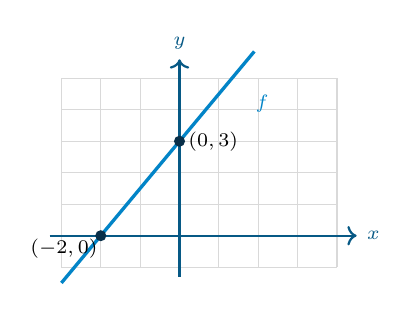
\begin{tikzpicture}[x=0.5cm,y=0.4cm]
\draw[gray!30,xstep=1,ystep=1] (-3,-1) grid (4,5);
\draw[->,thick,mainc] (-3.3,0)--(4.5,0) node[right,font=\scriptsize]{$x$};
\draw[->,thick,mainc] (0,-1.3)--(0,5.6) node[above,font=\scriptsize]{$y$};
\draw[accc,very thick] (-3,-1.5)--(1.9,5.85);
\fill[deepc] (-2,0) circle (2pt) (0,3) circle (2pt);
\node[font=\scriptsize,below left,inner sep=1pt] at (-2,0) {$(-2,0)$};
\node[font=\scriptsize,right,inner sep=3pt] at (0,3) {$(0,3)$};
\node[font=\scriptsize,accc] at (2.1,4.2) {$f$};
\end{tikzpicture}}}{\pil{$9$}{$10$}{$15$}{$12$}{$18$}}
\soal{Perhatikan lima grafik berikut. Grafik manakah yang \textbf{bukan} grafik sebuah fungsi $y=f(x)$ dengan $x$ sebagai variabel bebas?\par\smallskip
\centering
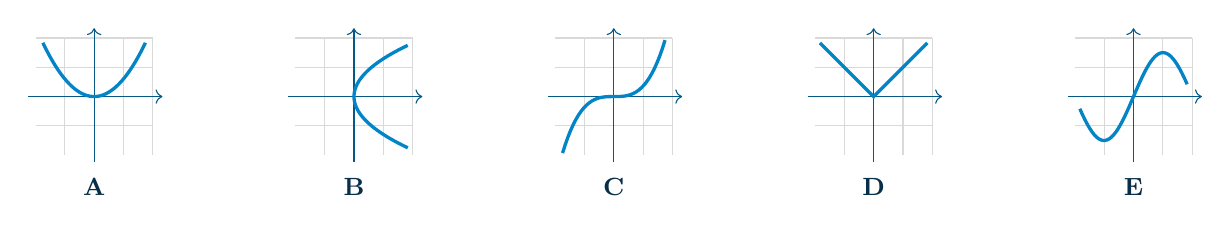
\begin{tikzpicture}[x=0.62cm,y=0.62cm]
\foreach \k/\L in {0/A,1/B,2/C,3/D,4/E}{
 \begin{scope}[xshift=\k*3.3cm]
 \draw[gray!30,step=0.6] (-1.2,-1.2) grid (1.2,1.2);
 \draw[->,mainc] (-1.35,0)--(1.4,0); \draw[->,mainc] (0,-1.35)--(0,1.4);
 \node[font=\small\bfseries,deepc] at (0,-1.85) {\L};
 \end{scope}}
\begin{scope}[xshift=0cm]\draw[accc,very thick,domain=-1.05:1.05,samples=40] plot (\x,{\x*\x});\end{scope}
\begin{scope}[xshift=3.3cm]\draw[accc,very thick,domain=-1.05:1.05,samples=40] plot ({\x*\x},{\x});\end{scope}
\begin{scope}[xshift=6.6cm]\draw[accc,very thick,domain=-1.05:1.05,samples=40] plot (\x,{\x*\x*\x});\end{scope}
\begin{scope}[xshift=9.9cm]\draw[accc,very thick] (-1.1,1.1)--(0,0)--(1.1,1.1);\end{scope}
\begin{scope}[xshift=13.2cm]\draw[accc,very thick,domain=-1.1:1.1,samples=60] plot (\x,{0.9*sin(\x*2.6 r)});\end{scope}
\end{tikzpicture}\par\smallskip\raggedright}{\pil{A}{B}{C}{D}{E}}
\soal{Suhu air pada sebuah pemanas naik secara linear terhadap waktu. Pada menit ke-$2$ suhunya $30^\circ$C dan pada menit ke-$5$ suhunya $48^\circ$C. Suhu air pada menit ke-$9$ adalah \dots.}{\pil{$54^\circ$C}{$60^\circ$C}{$66^\circ$C}{$78^\circ$C}{$72^\circ$C}}

\tingkat{Tingkat Sedang}{soal 6 sampai 10}
\soal{\gbr{Fungsi $f(x)=x^2-4x+1$ dengan domain $-1\le x\le4$ digambarkan seperti pada gambar. Selisih nilai maksimum dan nilai minimum $f$ pada domain tersebut adalah \dots.}{%
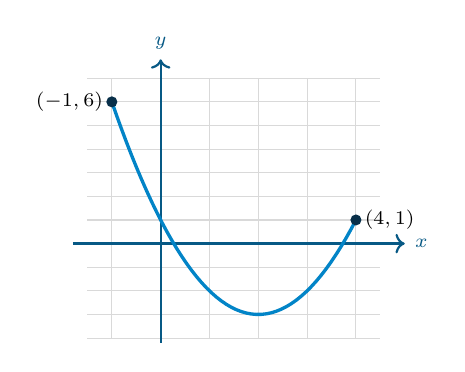
\begin{tikzpicture}[x=0.62cm,y=0.3cm]
\draw[gray!30,xstep=1,ystep=1] (-1.5,-4) grid (4.5,7);
\draw[->,thick,mainc] (-1.8,0)--(5,0) node[right,font=\scriptsize]{$x$};
\draw[->,thick,mainc] (0,-4.2)--(0,7.8) node[above,font=\scriptsize]{$y$};
\draw[accc,very thick,domain=-1:4,samples=50] plot (\x,{\x*\x-4*\x+1});
\fill[deepc] (-1,6) circle (2pt) (4,1) circle (2pt);
\node[font=\scriptsize,left,inner sep=3pt] at (-1,6) {$(-1,6)$};
\node[font=\scriptsize,right,inner sep=3pt] at (4,1) {$(4,1)$};
\end{tikzpicture}}}{\pil{$5$}{$6$}{$7$}{$9$}{$11$}}
\soal{Diketahui $f(x)=2x+3$ dan $(f\circ g)(x)=6x-1$. Nilai $g^{-1}(10)$ adalah \dots.}{\pil{$2$}{$3$}{$6$}{$8$}{$4$}}
\soal{\gbr{Fungsi $f$ hanya terdefinisi pada $-2\le x\le2$ dengan grafik pada gambar. Grafik $g(x)=-2f(x-1)+3$ mencapai titik terendahnya di \dots.}{%
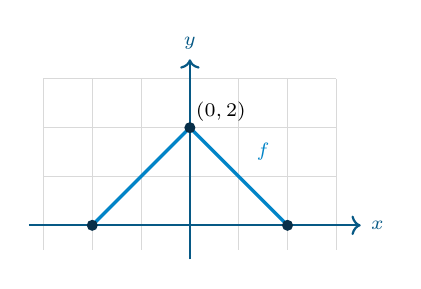
\begin{tikzpicture}[x=0.62cm,y=0.62cm]
\draw[gray!30,xstep=1,ystep=1] (-3,-0.5) grid (3,3);
\draw[->,thick,mainc] (-3.3,0)--(3.5,0) node[right,font=\scriptsize]{$x$};
\draw[->,thick,mainc] (0,-0.7)--(0,3.4) node[above,font=\scriptsize]{$y$};
\draw[accc,very thick] (-2,0)--(0,2)--(2,0);
\fill[deepc] (-2,0) circle (2pt) (0,2) circle (2pt) (2,0) circle (2pt);
\node[font=\scriptsize,above right,inner sep=2pt] at (0,2) {$(0,2)$};
\node[font=\scriptsize,accc] at (1.5,1.5) {$f$};
\end{tikzpicture}}}{\pilx{$(-1,-1)$}{$(1,7)$}{$(1,-1)$}{$(-1,7)$}{$(1,1)$}}
\soal{Tingkat intensitas bunyi dinyatakan $L=10\log\dfrac{I}{I_0}$ dB. Satu mesin menghasilkan bunyi $70$ dB. Jika empat mesin identik dinyalakan bersamaan (intensitas bunyi dijumlahkan) dan $\log2=0{,}3$, tingkat intensitas bunyi totalnya adalah \dots.}{\pil{$72$ dB}{$74$ dB}{$80$ dB}{$76$ dB}{$82$ dB}}
\soal{\gbr{Sebuah jasa kurir menetapkan biaya kirim (dalam ribuan rupiah) seperti pada grafik, dengan pola kenaikan yang terus berlanjut untuk jarak berikutnya. Biaya pengiriman untuk jarak $7{,}3$ km adalah \dots.}{%
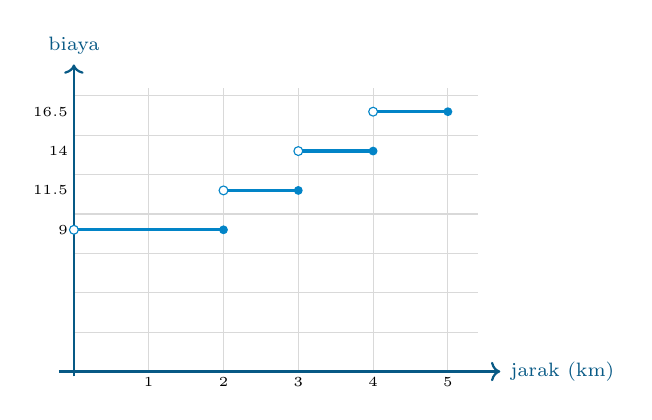
\begin{tikzpicture}[x=0.95cm,y=0.2cm]
\draw[gray!30,xstep=1,ystep=2.5] (0,0) grid (5.4,18);
\draw[->,thick,mainc] (-0.2,0)--(5.7,0) node[right,font=\scriptsize]{jarak (km)};
\draw[->,thick,mainc] (0,-0.3)--(0,19.5) node[above,font=\scriptsize]{biaya};
\foreach \a/\b/\v in {0/2/9,2/3/11.5,3/4/14,4/5/16.5}{
 \draw[accc,very thick] (\a,\v)--(\b,\v);
 \draw[accc,fill=white] (\a,\v) circle (1.6pt);
 \fill[accc] (\b,\v) circle (1.6pt);}
\foreach \v in {9,11.5,14,16.5}{\node[font=\tiny,left,inner sep=2pt] at (0,\v) {$\v$};}
\foreach \k in {1,...,5}{\node[font=\tiny,below,inner sep=2pt] at (\k,0) {$\k$};}
\end{tikzpicture}}}{\pil{Rp21.500}{Rp22.250}{Rp24.000}{Rp26.500}{Rp28.000}}

\tingkat{Tingkat Sulit}{soal 11 sampai 15, setara UTBK}
\soal{\gbr{Parabola pada gambar memotong sumbu-$x$ di $(-1,0)$ dan $(3,0)$, serta memotong sumbu-$y$ di $(0,3)$. Garis $y=1$ memotong parabola di titik $A$ dan $B$. Panjang ruas $AB$ adalah \dots.}{%
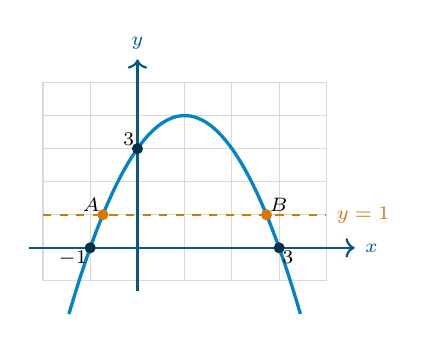
\begin{tikzpicture}[x=0.6cm,y=0.42cm]
\draw[gray!30,xstep=1,ystep=1] (-2,-1) grid (4,5);
\draw[->,thick,mainc] (-2.3,0)--(4.6,0) node[right,font=\scriptsize]{$x$};
\draw[->,thick,mainc] (0,-1.3)--(0,5.7) node[above,font=\scriptsize]{$y$};
\draw[accc,very thick,domain=-1.45:3.45,samples=60] plot (\x,{-\x*\x+2*\x+3});
\draw[warmc,thick,dashed] (-2,1)--(4,1) node[right,font=\scriptsize]{$y=1$};
\fill[deepc] (-1,0) circle (2pt) (3,0) circle (2pt) (0,3) circle (2pt);
\node[font=\scriptsize,below left,inner sep=1pt] at (-1,0) {$-1$};
\node[font=\scriptsize,below right,inner sep=1pt] at (3,0) {$3$};
\node[font=\scriptsize,above left,inner sep=1pt] at (0,3) {$3$};
\fill[warmc] (-0.732,1) circle (2pt) (2.732,1) circle (2pt);
\node[font=\scriptsize,above left,inner sep=1pt] at (-0.732,1) {$A$};
\node[font=\scriptsize,above right,inner sep=1pt] at (2.732,1) {$B$};
\end{tikzpicture}}}{\pil{$2\sqrt3$}{$2\sqrt2$}{$4$}{$2\sqrt5$}{$2\sqrt6$}}
\soal{Fungsi $f:\R\setminus\{0\}\to\R$ memenuhi $f(x)+2f\!\left(\dfrac1x\right)=3x$ untuk semua $x\neq0$. Nilai $x>0$ yang memenuhi $f(x)=0$ adalah \dots.}{\pil{$1$}{$2$}{$\sqrt3$}{$\sqrt2$}{$2\sqrt2$}}
\soal{Diketahui $f(x)=|x-2|$. Jumlah semua nilai $x$ yang memenuhi $(f\circ f)(x)=1$ adalah \dots.}{\pil{$4$}{$6$}{$8$}{$10$}{$12$}}
\soal{\gbr{Suhu sebuah kota (dalam $^\circ$C) selama sehari dimodelkan oleh fungsi kosinus. Pukul $14.00$ suhu mencapai maksimum $32^\circ$C dan pukul $02.00$ mencapai minimum $24^\circ$C (lihat gambar, $t$ dalam jam sejak pukul $00.00$). Selama $0\le t\le24$, suhu kota tersebut paling sedikit $30^\circ$C selama \dots\ jam.}{%
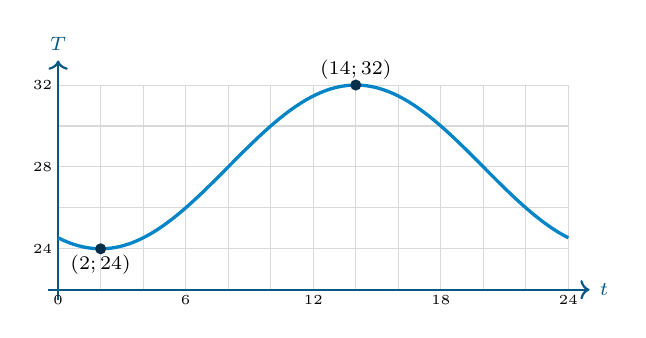
\begin{tikzpicture}[x=0.27cm,y=0.26cm]
\draw[gray!30,xstep=2,ystep=2] (0,0) grid (24,10);
\draw[->,thick,mainc] (-0.5,0)--(25,0) node[right,font=\scriptsize]{$t$};
\draw[->,thick,mainc] (0,-0.5)--(0,11.2) node[above,font=\scriptsize]{$T$};
\draw[accc,very thick,domain=0:24,samples=100] plot (\x,{6+4*cos((pi*(\x-14)/12) r)});
\fill[deepc] (14,10) circle (2pt) (2,2) circle (2pt);
\node[font=\scriptsize,above,inner sep=2pt] at (14,10) {$(14;32)$};
\node[font=\scriptsize,below,inner sep=2pt] at (2,2) {$(2;24)$};
\foreach \t in {0,6,12,18,24}{\node[font=\tiny,below,inner sep=2pt] at (\t,0) {$\t$};}
\foreach \y/\l in {2/24,6/28,10/32}{\node[font=\tiny,left,inner sep=2pt] at (0,\y) {$\l$};}
\end{tikzpicture}}}{\pil{$4$}{$6$}{$10$}{$12$}{$8$}}
\soal{Diketahui $f(x)=\dfrac{ax+b}{x-2}$ dengan $x\neq2$. Jika $f(f(x))=x$ untuk semua $x$ pada domainnya dan $f(1)=-5$, nilai $ab$ adalah \dots.}{\pil{$2$}{$5$}{$6$}{$8$}{$10$}}

\tingkat{Tingkat HOTS}{soal 16 sampai 20, penalaran tingkat tinggi gaya UTBK}
\soal{Apakah fungsi $f(x)=x^2+px+q$ dengan domain $[1,\infty)$ merupakan fungsi injektif?
\begin{enumerate}[label=(\arabic*),leftmargin=1.8em,itemsep=0pt,topsep=2pt]
\item $q=5$.
\item Grafik $f$ mencapai nilai minimum di $x=1$.
\end{enumerate}}{\begin{tabularx}{\linewidth}{@{}lX@{}}
\textbf{A.} & Pernyataan (1) SAJA cukup untuk menjawab pertanyaan, tetapi pernyataan (2) SAJA tidak cukup.\\
\textbf{B.} & Pernyataan (2) SAJA cukup untuk menjawab pertanyaan, tetapi pernyataan (1) SAJA tidak cukup.\\
\textbf{C.} & DUA pernyataan BERSAMA-SAMA cukup untuk menjawab pertanyaan, tetapi SATU pernyataan SAJA tidak cukup.\\
\textbf{D.} & Pernyataan (1) SAJA cukup dan pernyataan (2) SAJA cukup untuk menjawab pertanyaan.\\
\textbf{E.} & Pernyataan (1) dan pernyataan (2) tidak cukup untuk menjawab pertanyaan.
\end{tabularx}}
\soal{\gbr{Gambar menunjukkan grafik $f:\R\to\R$ dengan $f(x)=x^2-2|x|$. Tentukan nilai kebenaran tiga pernyataan berikut (B = benar, S = salah), berurutan dari (i) sampai (iii).\par\smallskip
(i) $f$ adalah fungsi genap.\par
(ii) $f:\R\to\R$ merupakan fungsi surjektif.\par
(iii) Jika domain $f$ dibatasi pada $[1,\infty)$, $f$ menjadi fungsi injektif.}{%
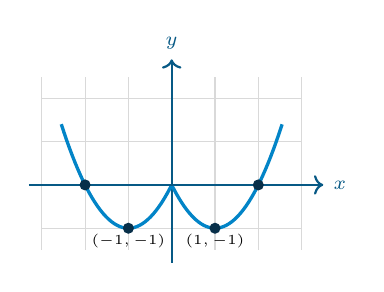
\begin{tikzpicture}[x=0.55cm,y=0.55cm]
\draw[gray!30,xstep=1,ystep=1] (-3,-1.5) grid (3,2.5);
\draw[->,thick,mainc] (-3.3,0)--(3.5,0) node[right,font=\scriptsize]{$x$};
\draw[->,thick,mainc] (0,-1.8)--(0,2.9) node[above,font=\scriptsize]{$y$};
\draw[accc,very thick,domain=-2.55:2.55,samples=80] plot (\x,{\x*\x-2*abs(\x)});
\fill[deepc] (-1,-1) circle (2pt) (1,-1) circle (2pt) (-2,0) circle (2pt) (2,0) circle (2pt);
\node[font=\tiny,below,inner sep=2pt] at (1,-1) {$(1,-1)$};
\node[font=\tiny,below,inner sep=2pt] at (-1,-1) {$(-1,-1)$};
\end{tikzpicture}}}{\pilx{B, B, B}{B, B, S}{B, S, B}{S, B, B}{S, S, S}}
\soal{\gbr{Sebuah lintasan lari berbentuk persegi panjang dengan dua setengah lingkaran di sisi-sisi lebarnya (lihat gambar). Panjang lintasan (tepi luar) adalah $400$ m. Luas maksimum daerah persegi panjang di tengah lintasan adalah \dots\ m$^2$.\par\smallskip\footnotesize (Petunjuk: nyatakan luas dalam jari-jari setengah lingkaran $r$.)}{%
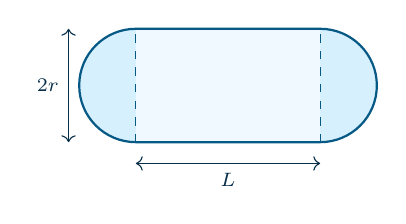
\begin{tikzpicture}[scale=0.9]
\fill[softbg] (0,0) rectangle (2.6,1.6);
\fill[skyl!60] (0,1.6) arc (90:270:0.8) -- cycle;
\fill[skyl!60] (2.6,0) arc (-90:90:0.8) -- cycle;
\draw[mainc,thick] (0,1.6) arc (90:270:0.8) -- (2.6,0) arc (-90:90:0.8) -- cycle;
\draw[mainc,thin,dashed] (0,0)--(0,1.6) (2.6,0)--(2.6,1.6);
\draw[<->,deepc] (0,-0.3)--(2.6,-0.3) node[midway,below,font=\scriptsize]{$L$};
\draw[<->,deepc] (-0.95,0)--(-0.95,1.6) node[midway,left,font=\scriptsize]{$2r$};
\end{tikzpicture}}}{\pil{$\dfrac{10.000}{\pi}$}{$\dfrac{20.000}{\pi}$}{$\dfrac{40.000}{\pi}$}{$\dfrac{5.000}{\pi}$}{$20.000\pi$}}
\soal{\gbr{Persamaan $\left\lfloor x\right\rfloor=\dfrac{2x-1}{3}$ dapat dipandang sebagai perpotongan grafik fungsi tangga $y=\lfloor x\rfloor$ dengan garis $y=\frac{2x-1}{3}$ (lihat gambar). Jumlah semua nilai $x$ yang memenuhi persamaan tersebut adalah \dots.}{%
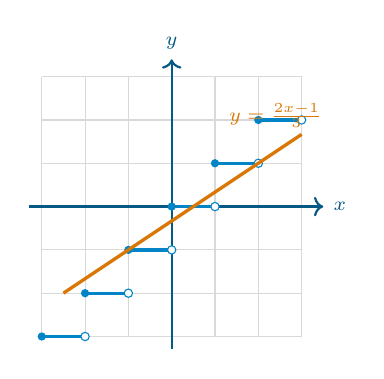
\begin{tikzpicture}[x=0.55cm,y=0.55cm]
\draw[gray!30,xstep=1,ystep=1] (-3,-3) grid (3,3);
\draw[->,thick,mainc] (-3.3,0)--(3.5,0) node[right,font=\scriptsize]{$x$};
\draw[->,thick,mainc] (0,-3.3)--(0,3.4) node[above,font=\scriptsize]{$y$};
\foreach \n in {-3,-2,-1,0,1,2}{
 \draw[accc,very thick] (\n,\n)--(\n+1,\n);
 \fill[accc] (\n,\n) circle (1.5pt);
 \draw[accc,fill=white] (\n+1,\n) circle (1.5pt);}
\draw[warmc,very thick] (-2.5,-2)--(3,1.667);
\node[font=\scriptsize,warmc] at (2.4,2.1) {$y=\frac{2x-1}{3}$};
\end{tikzpicture}}}{\pil{$\dfrac12$}{$-1$}{$\dfrac32$}{$0$}{$-\dfrac12$}}
\soal{\gbr{Dua akun media sosial memiliki pertumbuhan pengikut pada hari ke-$n$ ($n=0,1,2,\dots$): akun $A$ sebanyak $A(n)=1.000+300n$ dan akun $B$ sebanyak $B(n)=50\cdot2^n$ (lihat gambar, sumbu tegak dalam ribuan). Hingga akun $B$ menyalip akun $A$, selisih terbesar $A(n)-B(n)$ yang terjadi pada hari bilangan bulat adalah \dots.}{%
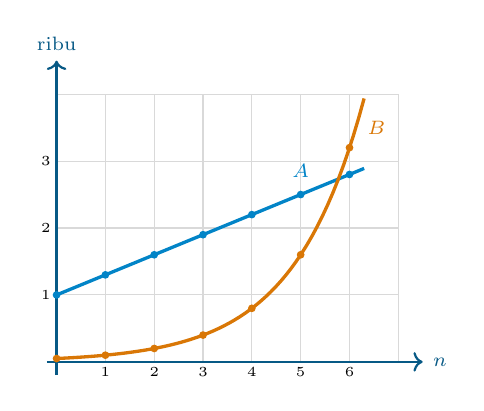
\begin{tikzpicture}[x=0.62cm,y=0.85cm]
\draw[gray!30,xstep=1,ystep=1] (0,0) grid (7,4);
\draw[->,thick,mainc] (-0.2,0)--(7.5,0) node[right,font=\scriptsize]{$n$};
\draw[->,thick,mainc] (0,-0.2)--(0,4.5) node[above,font=\scriptsize]{ribu};
\draw[accc,very thick] (0,1)--(6.3,2.89);
\draw[warmc,very thick,domain=0:6.3,samples=60] plot (\x,{0.05*2^\x});
\foreach \n in {0,...,6}{\fill[accc] (\n,{1+0.3*\n}) circle (1.4pt); \fill[warmc] (\n,{0.05*2^\n}) circle (1.4pt);}
\node[font=\scriptsize,accc] at (5.0,2.85) {$A$};
\node[font=\scriptsize,warmc] at (6.55,3.5) {$B$};
\foreach \n in {1,...,6}{\node[font=\tiny,below,inner sep=2pt] at (\n,0) {$\n$};}
\foreach \y in {1,2,3}{\node[font=\tiny,left,inner sep=2pt] at (0,\y) {$\y$};}
\end{tikzpicture}}}{\pil{$1.200$}{$1.500$}{$1.800$}{$1.400$}{$1.600$}}

% =====================================================================
\bagian{B. Isian Singkat}{5 soal $\times$ 4 poin = 20 poin. Tuliskan hanya jawaban akhir.}

\tingkat{Tingkat Sedang}{soal 1 dan 2}
\soal{Fungsi $f(x)=\dfrac{2x+1}{x-3}$ memiliki domain $x\ge4$. Jumlah semua bilangan bulat yang berada pada range $f$ adalah \dots.}{\jwb}
\soal{Grafik $y=f(x)$ melalui titik $(2,5)$. Grafik $y=-3f(2x-4)+1$ pasti melalui titik $(a,b)$. Nilai $a+b$ adalah \dots.}{\jwb}

\tingkat{Tingkat Sulit}{soal 3 sampai 5}
\soal{Banyak bilangan bulat $n$ dengan $1\le n\le100$ sehingga $\left\lfloor\sqrt n\right\rfloor$ habis dibagi $3$ adalah \dots.}{\jwb}
\soal{\gbr{Grafik $y=f(x)$ pada $0\le x\le4$ berbentuk garis patah seperti pada gambar, dengan titik-titik sudut $(0,0)$, $(1,2)$, $(2,0)$, $(3,2)$, dan $(4,0)$. Banyak nilai $x\in[0,4]$ yang memenuhi $f(f(x))=1$ adalah \dots.}{%
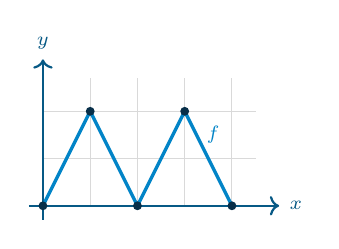
\begin{tikzpicture}[x=0.6cm,y=0.6cm]
\draw[gray!30,xstep=1,ystep=1] (0,0) grid (4.5,2.7);
\draw[->,thick,mainc] (-0.3,0)--(5,0) node[right,font=\scriptsize]{$x$};
\draw[->,thick,mainc] (0,-0.3)--(0,3.1) node[above,font=\scriptsize]{$y$};
\draw[accc,very thick] (0,0)--(1,2)--(2,0)--(3,2)--(4,0);
\fill[deepc] (0,0) circle (1.6pt) (1,2) circle (1.6pt) (2,0) circle (1.6pt) (3,2) circle (1.6pt) (4,0) circle (1.6pt);
\node[font=\scriptsize,accc] at (3.6,1.5) {$f$};
\end{tikzpicture}}}{\jwb}
\soal{Dua benda panas didinginkan. Suhu benda $P$ (dalam $^\circ$C) setelah $t$ menit adalah $P(t)=20+60\cdot2^{-t/5}$, sedangkan suhu benda $Q$ adalah $Q(t)=20+30\cdot2^{-t/10}$. Pada suatu saat $t>0$ kedua benda memiliki suhu yang sama. Suhu tersebut adalah \dots\ $^\circ$C.}{\jwb}

% =====================================================================
\Needspace{16\baselineskip}
\bagian{C. Uraian (Essay)}{5 soal $\times$ 8 poin = 40 poin. Tuliskan langkah penyelesaian dengan lengkap.}

\tingkat{Tingkat Sedang}{soal 1 dan 2}
\soal{\gbr{Dua layanan pengiriman paket menetapkan tarif berdasarkan berat $w$ kg, dengan pecahan kilogram dibulatkan ke atas. Layanan $A$: Rp12.000 untuk $1$ kg pertama dan Rp7.000 untuk setiap kg berikutnya. Layanan $B$: Rp9.500 per kg tanpa biaya awal. Grafik kedua tarif untuk $0<w\le4$ ditunjukkan pada gambar (sumbu tegak dalam ribuan rupiah).\par\smallskip
(a) Tuliskan rumus biaya $A(w)$ dan $B(w)$ dengan memakai $\lceil w\rceil$.\par
(b) Hitung biaya mengirim paket $3{,}2$ kg dengan masing-masing layanan.\par
(c) Tentukan semua berat $w$ yang membuat layanan $A$ lebih murah daripada $B$.\par
(d) Berapa rupiah penghematan jika paket $7{,}5$ kg dikirim lewat layanan yang lebih murah?}{%
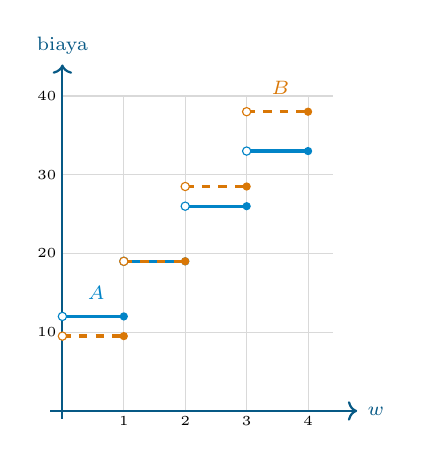
\begin{tikzpicture}[x=0.78cm,y=0.1cm]
\draw[gray!30,xstep=1,ystep=10] (0,0) grid (4.4,40);
\draw[->,thick,mainc] (-0.2,0)--(4.8,0) node[right,font=\scriptsize]{$w$};
\draw[->,thick,mainc] (0,-1)--(0,44) node[above,font=\scriptsize]{biaya};
\foreach \a/\b/\v in {0/1/12,1/2/19,2/3/26,3/4/33}{
 \draw[accc,very thick] (\a,\v)--(\b,\v);
 \draw[accc,fill=white] (\a,\v) circle (1.5pt); \fill[accc] (\b,\v) circle (1.5pt);}
\foreach \a/\b/\v in {0/1/9.5,1/2/19,2/3/28.5,3/4/38}{
 \draw[warmc,very thick,dashed] (\a,\v)--(\b,\v);
 \draw[warmc,fill=white] (\a,\v) circle (1.5pt); \fill[warmc] (\b,\v) circle (1.5pt);}
\node[font=\scriptsize,accc] at (0.55,15) {$A$}; \node[font=\scriptsize,warmc] at (3.55,41) {$B$};
\foreach \k in {1,2,3,4}{\node[font=\tiny,below,inner sep=2pt] at (\k,0) {$\k$};}
\foreach \y in {10,20,30,40}{\node[font=\tiny,left,inner sep=2pt] at (0,\y) {$\y$};}
\end{tikzpicture}}}{\poin{8}}
\soal{\gbr{Sebuah gerbang berbentuk busur parabola memiliki lebar dasar $8$ m dan tinggi maksimum $6$ m di tengahnya (lihat gambar). Letakkan titik asal di tengah dasar gerbang.\par\smallskip
(a) Tentukan fungsi kuadrat $y=h(x)$ yang memodelkan lengkung gerbang.\par
(b) Berapa tinggi gerbang pada jarak $1$ m dari tepi dasar?\par
(c) Sebuah truk berlebar $3$ m dan bertinggi $5$ m melewati tengah gerbang. Apakah truk dapat lewat? Jelaskan dengan perhitungan.\par
(d) Untuk truk setinggi $4{,}5$ m, berapa lebar maksimum truk agar dapat lewat tepat di bawah gerbang?}{%
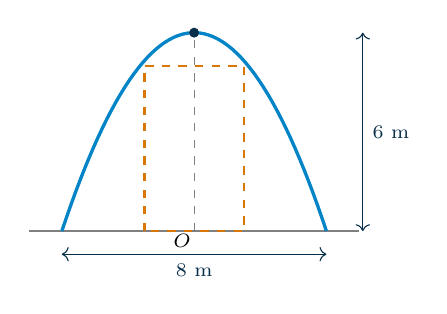
\begin{tikzpicture}[x=0.42cm,y=0.42cm]
\draw[gray,thick] (-5,0)--(5,0);
\draw[accc,very thick,domain=-4:4,samples=60] plot (\x,{6-3/8*\x*\x});
\draw[warmc,thick,dashed] (-1.5,0) rectangle (1.5,5);
\draw[<->,deepc] (-4,-0.7)--(4,-0.7) node[midway,below,font=\scriptsize]{$8$ m};
\draw[<->,deepc] (5.1,0)--(5.1,6) node[midway,right,font=\scriptsize]{$6$ m};
\draw[gray,dashed] (0,0)--(0,6);
\fill[deepc] (0,6) circle (1.8pt);
\node[font=\scriptsize,below left,inner sep=1pt] at (0,0) {$O$};
\end{tikzpicture}}}{\poin{8}}

\tingkat{Tingkat Sulit}{soal 3 dan 4}
\soal{\gbr{Diketahui $f(x)=\sqrt{x+3}-1$ dengan domain $x\ge-3$. Gambar memperlihatkan grafik $f$ (biru), grafik $f^{-1}$ (oranye), dan garis $y=x$ (putus-putus).\par\smallskip
(a) Tentukan range $f$, lalu jelaskan mengapa $f:[-3,\infty)\to[-1,\infty)$ merupakan fungsi bijektif.\par
(b) Tentukan $f^{-1}(x)$ beserta domain dan rangenya.\par
(c) Tentukan koordinat titik potong grafik $f$ dan $f^{-1}$. Periksa apakah ada akar palsu.\par
(d) Buktikan bahwa karena $f$ fungsi naik, setiap titik potong grafik $f$ dan $f^{-1}$ terletak pada garis $y=x$.}{%
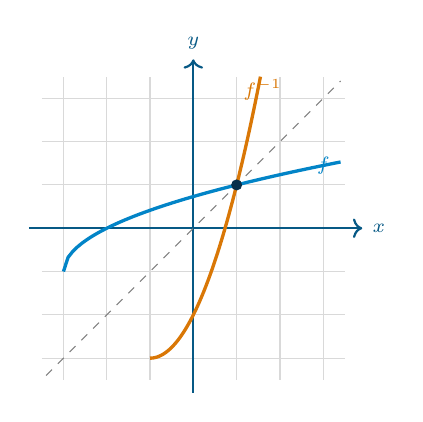
\begin{tikzpicture}[x=0.55cm,y=0.55cm]
\draw[gray!30,xstep=1,ystep=1] (-3.5,-3.5) grid (3.5,3.5);
\draw[->,thick,mainc] (-3.8,0)--(3.9,0) node[right,font=\scriptsize]{$x$};
\draw[->,thick,mainc] (0,-3.8)--(0,3.9) node[above,font=\scriptsize]{$y$};
\draw[gray,dashed] (-3.4,-3.4)--(3.4,3.4);
\draw[accc,very thick,domain=-3:3.4,samples=60] plot (\x,{sqrt(\x+3)-1});
\draw[warmc,very thick,domain=-1:1.55,samples=60] plot (\x,{(\x+1)*(\x+1)-3});
\fill[deepc] (1,1) circle (2pt);
\node[font=\scriptsize,accc] at (3.0,1.45) {$f$}; \node[font=\scriptsize,warmc] at (1.6,3.2) {$f^{-1}$};
\end{tikzpicture}}}{\poin{8}}
\soal{\gbr{Katup (pentil) pada roda sebuah sepeda berjari-jari $35$ cm berputar bersama roda. Roda berputar $2$ kali tiap detik dan pada $t=0$ katup berada di titik terendah (menyentuh tanah). Tinggi katup dari tanah dimodelkan $h(t)=35-35\cos(4\pi t)$ cm.\par\smallskip
(a) Jelaskan arti angka $35$, $35$, dan $4\pi$ pada model tersebut, lalu tentukan periodenya.\par
(b) Kapan pertama kali katup berada pada ketinggian $52{,}5$ cm?\par
(c) Dalam satu putaran, berapa bagian waktu katup berada di atas $52{,}5$ cm?\par
(d) Tentukan kecepatan sepeda (dalam m/s dan km/jam) bila roda menggelinding tanpa slip; gunakan $\pi=\frac{22}{7}$.}{%
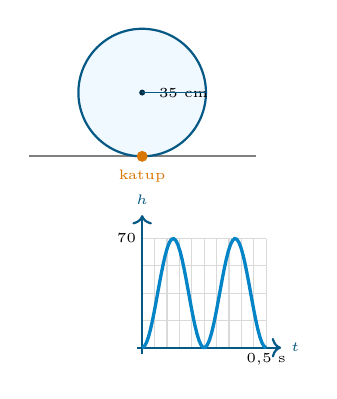
\begin{tikzpicture}[scale=0.9]
\draw[gray,thick] (-1.6,0)--(1.6,0);
\draw[mainc,thick,fill=softbg] (0,0.9) circle (0.9);
\fill[deepc] (0,0.9) circle (1.2pt);
\fill[warmc] (0,0) circle (2.2pt);
\node[font=\tiny,right] at (0.1,0.9) {$35$ cm};
\draw[mainc,thin] (0,0.9)--(0.9,0.9);
\node[font=\tiny,warmc,below] at (0,-0.05) {katup};
\begin{scope}[yshift=-2.7cm,x=0.14cm,y=0.022cm]
\draw[gray!30,xstep=1.25,ystep=17.5] (0,0) grid (12.5,70);
\draw[->,thick,mainc] (-0.5,0)--(14,0) node[right,font=\tiny]{$t$};
\draw[->,thick,mainc] (0,-4)--(0,85) node[above,font=\tiny]{$h$};
\draw[accc,very thick,domain=0:12.5,samples=60] plot (\x,{35-35*cos((pi*\x/6.25*2) r)});
\node[font=\tiny,left,inner sep=2pt] at (0,70) {$70$};
\node[font=\tiny,below,inner sep=2pt] at (12.5,0) {$0{,}5$ s};
\end{scope}
\end{tikzpicture}}}{\poin{8}}

\tingkat{Tingkat HOTS}{soal 5}
\soal{\gbr{Seorang pasien meminum antibiotik $200$ mg setiap $6$ jam. Kadar obat dalam darah meluruh secara eksponensial: setelah $6$ jam kadarnya tinggal separuh. Misalkan dosis pertama diminum pada $t=0$ dan kadar langsung naik sebesar $200$ mg setiap kali minum (lihat gambar, sumbu tegak dalam ratusan mg).\par\smallskip
(a) Tuliskan model kadar akibat satu dosis saja, $C(t)$, untuk $t\ge0$.\par
(b) Hitung kadar tepat sebelum dan tepat sesudah minum dosis kedua, lalu kadar tepat sesudah dosis ketiga.\par
(c) Tunjukkan bahwa kadar puncak sesudah dosis ke-$n$ adalah $P_n=400\left(1-2^{-n}\right)$. Mengapa kadar puncak tidak pernah mencapai $400$ mg?\par
(d) Berapa dosis paling sedikit agar kadar puncak melampaui $390$ mg? (Gunakan $2^5=32$ dan $2^6=64$.)}{%
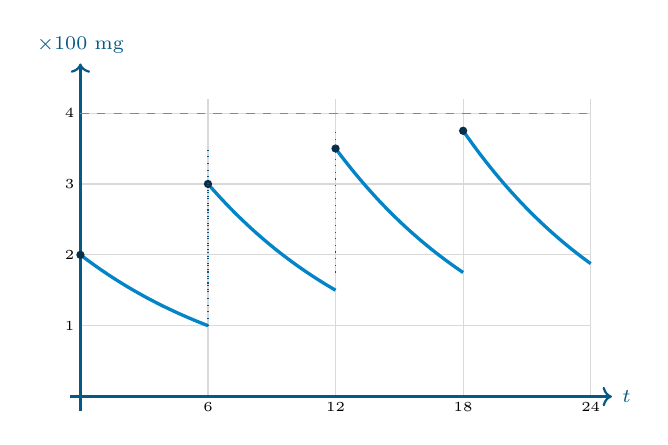
\begin{tikzpicture}[x=0.27cm,y=0.9cm]
\draw[gray!30,xstep=6,ystep=1] (0,0) grid (24,4.2);
\draw[->,thick,mainc] (-0.5,0)--(25,0) node[right,font=\scriptsize]{$t$};
\draw[->,thick,mainc] (0,-0.2)--(0,4.7) node[above,font=\scriptsize]{$\times100$ mg};
\draw[warmc,dashed] (0,4)--(24,4);
\foreach \k/\s in {0/2,1/3,2/3.5,3/3.75}{
 \draw[accc,very thick,domain={6*\k}:{6*\k+6},samples=30] plot (\x,{\s*2^(-(\x-6*\k)/6)});
 \fill[deepc] ({6*\k},\s) circle (1.5pt);}
\foreach \k/\a/\b in {1/1.5/3.5,2/1.75/3.75}{\draw[mainc,dotted] ({6*\k},\a)--({6*\k},\b);}
\draw[mainc,dotted] (6,1)--(6,3);
\foreach \t in {6,12,18,24}{\node[font=\tiny,below,inner sep=2pt] at (\t,0) {$\t$};}
\foreach \y in {1,2,3,4}{\node[font=\tiny,left,inner sep=2pt] at (0,\y) {$\y$};}
\end{tikzpicture}}}{\poin{8}}

% =====================================================================
\newpage
\bagian{Kunci Jawaban dan Pembahasan Singkat}{Untuk guru dan pembahasan mandiri}
\par\vspace{0.6em}{\bfseries\color{mainc}Kunci Pilihan Ganda}\par\vspace{0.3em}
\small
\begin{tabularx}{\linewidth}{@{}*{10}{>{\centering\arraybackslash}X}@{}}\hline \textbf{1} & \textbf{2} & \textbf{3} & \textbf{4} & \textbf{5} & \textbf{6} & \textbf{7} & \textbf{8} & \textbf{9} & \textbf{10}\\ \hline B & C & D & B & E & D & E & C & D & C\\ \hline\end{tabularx}\\[6pt]
\begin{tabularx}{\linewidth}{@{}*{10}{>{\centering\arraybackslash}X}@{}}\hline \textbf{11} & \textbf{12} & \textbf{13} & \textbf{14} & \textbf{15} & \textbf{16} & \textbf{17} & \textbf{18} & \textbf{19} & \textbf{20}\\ \hline A & D & C & E & C & B & C & B & E & B\\ \hline\end{tabularx}
\par\vspace{0.4em}{\bfseries\color{mainc}Kunci Isian Singkat:}\ \ 1) $42$\quad 2) $-11$\quad 3) $39$\quad 4) $8$\quad 5) $35$
\par\vspace{0.8em}{\bfseries\color{mainc}\normalsize Pembahasan Pilihan Ganda}\par\vspace{0.2em}
\small\begin{enumerate}[leftmargin=2em,itemsep=2pt,topsep=2pt]
\item[\textbf{1.}] \textbf{(B)} Syarat: $5-x\ge0\Rightarrow x\le5$ dan $x-1>0\Rightarrow x>1$. Domain $1<x\le5$ memuat bilangan bulat $2,3,4,5$, yaitu $4$ bilangan. (Jebakan: memasukkan $1$ atau membuang $5$.)
\item[\textbf{2.}] \textbf{(C)} $(g\circ f)(3)=g(5)=28$ dan $(f\circ g)(3)=f(12)=23$, sehingga selisihnya $5$. Hasil ini sekaligus menunjukkan $g\circ f\neq f\circ g$.
\item[\textbf{3.}] \textbf{(D)} Gradien $=\frac{3-0}{0-(-2)}=\frac32$, sehingga $f(x)=\frac32x+3$ dan $f(6)=9+3=12$.
\item[\textbf{4.}] \textbf{(B)} Uji garis vertikal: garis $x=c$ ($c>0$) pada grafik B memotong kurva di dua titik, sehingga satu nilai $x$ punya dua nilai $y$. Grafik B adalah $x=y^2$. Grafik A, C, D, dan E masing-masing dipotong paling banyak satu kali oleh garis vertikal.
\item[\textbf{5.}] \textbf{(E)} Laju kenaikan $\frac{48-30}{5-2}=6^\circ$C/menit, sehingga $T(t)=30+6(t-2)=6t+18$ dan $T(9)=72^\circ$C.
\item[\textbf{6.}] \textbf{(D)} Puncak di $x=2$ dengan $f(2)=-3$ (minimum), dan $2\in[-1,4]$. Ujung: $f(-1)=6$ dan $f(4)=1$, sehingga maksimum $6$. Selisih $6-(-3)=9$. (Jebakan: hanya membandingkan ujung, hasilnya $5$.)
\item[\textbf{7.}] \textbf{(E)} $(f\circ g)(x)=2g(x)+3=6x-1\Rightarrow g(x)=3x-2$ dan $g^{-1}(y)=\frac{y+2}3$. Jadi $g^{-1}(10)=4$.
\item[\textbf{8.}] \textbf{(C)} $f$ bernilai tertinggi $2$ di $x=0$. $f(x-1)$ menggeser grafik $1$ satuan ke \emph{kanan} sehingga puncaknya di $(1,2)$. Pengali $-2$ membalik dan meregangkan: $y=-2\cdot2=-4$, lalu $+3$ memberi $y=-1$. Jadi titik terendah $g$ adalah $(1,-1)$.
\item[\textbf{9.}] \textbf{(D)} Intensitas total $=4I$, sehingga $L=10\log\frac{4I}{I_0}=10\log4+10\log\frac{I}{I_0}=10(0{,}6)+70=76$ dB. (Jebakan: mengira $4\times70$ atau menambah $4$ dB.)
\item[\textbf{10.}] \textbf{(C)} Dari grafik: $9$ untuk $(0,2]$, lalu naik $2{,}5$ tiap km: $(2,3]\to11{,}5$; $(3,4]\to14$; $(4,5]\to16{,}5$; $(5,6]\to19$; $(6,7]\to21{,}5$; $(7,8]\to24$. Jarak $7{,}3$ km berada di $(7,8]$, sehingga biayanya Rp24.000. (Model: $C=9+2{,}5\lceil x-2\rceil$.)
\item[\textbf{11.}] \textbf{(A)} $y=a(x+1)(x-3)$; melalui $(0,3)$: $-3a=3\Rightarrow a=-1$, sehingga $y=-x^2+2x+3$. Dengan $y=1$: $x^2-2x-2=0\Rightarrow x=1\pm\sqrt3$. Maka $AB=(1+\sqrt3)-(1-\sqrt3)=2\sqrt3$.
\item[\textbf{12.}] \textbf{(D)} Substitusi $x\to\frac1x$: $f(\frac1x)+2f(x)=\frac3x$. Dari kedua persamaan: $f(x)=\frac2x-x$. Maka $f(x)=0\Rightarrow x^2=2\Rightarrow x=\sqrt2$ (untuk $x>0$).
\item[\textbf{13.}] \textbf{(C)} $(f\circ f)(x)=\big||x-2|-2\big|=1\Rightarrow|x-2|-2=\pm1\Rightarrow|x-2|=3$ atau $|x-2|=1$. Maka $x\in\{5,-1,3,1\}$ dan jumlahnya $8$.
\item[\textbf{14.}] \textbf{(E)} Garis tengah $28$, amplitudo $4$, periode $24$: $T(t)=28+4\cos\frac{\pi(t-14)}{12}$. $T\ge30\iff\cos\theta\ge\frac12$ dengan $\theta=\frac{\pi(t-14)}{12}$, yaitu $|\theta|\le\frac\pi3\iff|t-14|\le4$. Selang $10\le t\le18$ memiliki panjang $8$ jam.
\item[\textbf{15.}] \textbf{(C)} $f(f(x))=\dfrac{(a^2+b)x+(a-2)b}{(a-2)x+(b+4)}$. Agar sama dengan $x$ untuk semua $x$ diperlukan $a-2=0$, sehingga $a=2$ (syarat lain terpenuhi). Dari $f(1)=\frac{2+b}{-1}=-5$ diperoleh $b=3$. Jadi $ab=6$.
\item[\textbf{16.}] \textbf{(B)} Parabola dengan koefisien $x^2$ positif turun sebelum puncak dan naik setelahnya, puncak di $x=-\frac p2$. $f$ injektif pada $[1,\infty)$ jika dan hanya jika $-\frac p2\le1$. Pernyataan (1) tentang $q$ tidak mengubah letak puncak, sehingga tidak cukup. Pernyataan (2) berarti $-\frac p2=1$, sehingga $f$ naik di seluruh $[1,\infty)$ dan injektif. Hanya (2) cukup.
\item[\textbf{17.}] \textbf{(C)} Grafik simetris terhadap sumbu-$y$: (i) \textbf{B} ($f(-x)=f(x)$). Range $f$ adalah $[-1,\infty)$ sehingga (ii) \textbf{S} (nilai $y<-1$ tidak dicapai). Pada $x\ge1$, $f(x)=x^2-2x$ dengan puncak di $x=1$, jadi selalu naik dan (iii) \textbf{B}. Urutan: B, S, B.
\item[\textbf{18.}] \textbf{(B)} Keliling: $2L+2\pi r=400\Rightarrow L=200-\pi r$. Luas persegi panjang $=2r(200-\pi r)=400r-2\pi r^2$, maksimum di $r=\frac{400}{4\pi}=\frac{100}\pi$ dengan nilai $\frac{40.000}\pi-\frac{20.000}\pi=\frac{20.000}\pi$ m$^2$ (sekitar $6.364$ m$^2$ dengan $\pi=\frac{22}{7}$).
\item[\textbf{19.}] \textbf{(E)} Misalkan $n=\lfloor x\rfloor$, sehingga $n=\frac{2x-1}3\Rightarrow x=\frac{3n+1}2$. Syarat $n\le x<n+1$: $2n\le3n+1\Rightarrow n\ge-1$ dan $3n+1<2n+2\Rightarrow n<1$. Jadi $n=-1$ atau $0$ dengan $x=-1$ dan $x=\frac12$ (sesuai dua perpotongan pada gambar). Jumlahnya $-\frac12$.
\item[\textbf{20.}] \textbf{(B)} Selisih $d(n)=A(n)-B(n)=1.000+300n-50\cdot2^n$: $d(0)=950$, $d(1)=1.200$, $d(2)=1.400$, $d(3)=1.500$, $d(4)=1.400$, $d(5)=900$, $d(6)=-400$. Selisih terbesar $1.500$ pada hari ke-$3$, dan $B$ menyalip pada hari ke-$6$. (Jebakan: terkecoh memilih hari ke-$2$ atau ke-$4$ yang bernilai $1.400$.)
\end{enumerate}
\par\Needspace{6\baselineskip}\vspace{0.6em}{\bfseries\color{mainc}\normalsize Pembahasan Isian Singkat}\par\vspace{0.2em}
\small\begin{enumerate}[leftmargin=2em,itemsep=2pt,topsep=2pt]
\item[\textbf{1.}] \textbf{Jawaban: $42$.} $f(x)=\frac{2x+1}{x-3}=2+\frac7{x-3}$. Untuk $x\ge4$, $x-3\ge1$ sehingga $\frac7{x-3}\in(0,7]$ dan $f$ turun dari $f(4)=9$ mendekati $2$ tanpa mencapainya. Range $=(2,9]$ dengan bilangan bulat $3,4,\dots,9$, jumlahnya $42$.
\item[\textbf{2.}] \textbf{Jawaban: $-11$.} Titik $(2,5)$ pada $f$ berarti $f(2)=5$. Agar $f(2x-4)$ memakai nilai $f(2)$, haruskan $2x-4=2\Rightarrow x=3$. Maka $y=-3\cdot5+1=-14$. Titik $(3,-14)$ sehingga $a+b=-11$.
\item[\textbf{3.}] \textbf{Jawaban: $39$.} $\lfloor\sqrt n\rfloor=k\iff k^2\le n\le k^2+2k$ ($2k+1$ bilangan). $k$ kelipatan $3$: $k=3$ ($n=9,\dots,15$; $7$ bilangan), $k=6$ ($n=36,\dots,48$; $13$ bilangan), $k=9$ ($n=81,\dots,99$; $19$ bilangan). $n=100$ memberi $k=10$ (tidak). Total $7+13+19=39$.
\item[\textbf{4.}] \textbf{Jawaban: $8$.} Karena $f(x)\in[0,2]$, haruslah $y=f(x)$ memenuhi $f(y)=1$ dengan $y\in[0,2]$: pada $[0,2]$, $f(y)=1$ di $y=\frac12$ dan $y=\frac32$ (nilai $\frac52$ dan $\frac72$ di luar range). Untuk setiap nilai $c\in(0,2)$, persamaan $f(x)=c$ memiliki $4$ solusi di $[0,4]$ (satu pada tiap ruas garis). Jadi banyak solusi $=2\times4=8$.
\item[\textbf{5.}] \textbf{Jawaban: $35$.} Samakan: $60\cdot2^{-t/5}=30\cdot2^{-t/10}$. Misalkan $u=2^{-t/10}$, maka $2^{-t/5}=u^2$ dan $60u^2=30u\Rightarrow u=\frac12$ (karena $u>0$) sehingga $t=10$ menit. Suhu: $Q(10)=20+30\cdot\frac12=35$; cek $P(10)=20+60\cdot\frac14=35$.
\end{enumerate}
\par\Needspace{8\baselineskip}\vspace{0.6em}{\bfseries\color{mainc}\normalsize Pembahasan dan Pedoman Penskoran Uraian}\par\vspace{0.2em}
\small\begin{enumerate}[leftmargin=2em,itemsep=3pt,topsep=2pt]
\item[\textbf{1.}] (a) Jumlah kg yang ditagih adalah $\lceil w\rceil$. $A(w)=12.000+7.000(\lceil w\rceil-1)=5.000+7.000\lceil w\rceil$ dan $B(w)=9.500\lceil w\rceil$. (b) $w=3{,}2\Rightarrow\lceil w\rceil=4$: $A=5.000+28.000=\text{Rp}33.000$ dan $B=\text{Rp}38.000$. (c) $A<B\iff5.000+7.000n<9.500n\iff n>2$ dengan $n=\lceil w\rceil$. Jadi $\lceil w\rceil\ge3$, yaitu $w>2$ kg (pada $n=2$ keduanya Rp19.000). (d) $w=7{,}5\Rightarrow n=8$: $A=5.000+56.000=\text{Rp}61.000$ dan $B=\text{Rp}76.000$. Layanan $A$ lebih murah dan penghematannya Rp15.000. \\ \textit{Penskoran: tiap bagian 2 poin.}
\item[\textbf{2.}] (a) Titik puncak $(0,6)$ dan akar $x=\pm4$: $h(x)=6-kx^2$ dengan $h(4)=0\Rightarrow k=\frac{6}{16}=\frac38$, sehingga $h(x)=6-\frac38x^2$. (b) Jarak $1$ m dari tepi berarti $x=3$: $h(3)=6-\frac{27}8=\frac{21}8=2{,}625$ m. (c) Truk lebar $3$ m berarti tepinya di $x=\pm1{,}5$: $h(1{,}5)=6-\frac38\cdot\frac94=\frac{165}{32}\approx5{,}16$ m $>5$ m, sehingga truk dapat lewat (selisih sekitar $16$ cm). (d) $h(x)=4{,}5\Rightarrow\frac38x^2=1{,}5\Rightarrow x^2=4\Rightarrow x=\pm2$. Lebar maksimum $=2\cdot2=4$ m. \\ \textit{Penskoran: (a) 3 poin; (b) 1 poin; (c) 2 poin; (d) 2 poin.}
\item[\textbf{3.}] (a) Karena $\sqrt{x+3}\ge0$, nilai $f(x)\ge-1$ dan nilai $-1$ dicapai di $x=-3$. Untuk setiap $y\ge-1$, persamaan $\sqrt{x+3}-1=y$ memberi $x=(y+1)^2-3\ge-3$, jadi $f$ surjektif ke $[-1,\infty)$. $f$ injektif karena $\sqrt{\cdot}$ naik tegas ($x_1<x_2\Rightarrow f(x_1)<f(x_2)$). Jadi $f$ bijektif. (b) $y=\sqrt{x+3}-1\Rightarrow x=(y+1)^2-3$, sehingga $f^{-1}(x)=(x+1)^2-3$ dengan domain $x\ge-1$ dan range $y\ge-3$. (c) Karena titik potong ada di garis $y=x$ (lihat (d)): $\sqrt{x+3}-1=x\Rightarrow\sqrt{x+3}=x+1\Rightarrow x^2+x-2=0\Rightarrow x=1$ atau $x=-2$. Syarat $x+1\ge0$ membuat $x=-2$ akar palsu. Titik potong: $(1,1)$. (d) Misalkan $(a,b)$ terletak pada kedua grafik: $b=f(a)$ dan $b=f^{-1}(a)$ sehingga $f(b)=a$. Jika $a<b$, karena $f$ naik maka $f(a)<f(b)$, yaitu $b<a$ (kontradiksi). Jika $a>b$, diperoleh $b>a$ (kontradiksi). Jadi $a=b$. \\ \textit{Penskoran: tiap bagian 2 poin.}
\item[\textbf{4.}] (a) Angka $35$ pertama adalah tinggi garis tengah (tinggi pusat roda), angka $35$ kedua (koefisien kosinus) adalah amplitudo atau jari-jari roda, dan $4\pi$ adalah $\omega=\frac{2\pi}{T}$ (sudut yang ditempuh tiap detik, yaitu $2$ putaran $\times2\pi$). Periode $T=\frac{2\pi}{4\pi}=\frac12$ detik. (b) $35-35\cos4\pi t=52{,}5\Rightarrow\cos4\pi t=-\frac12\Rightarrow4\pi t=\frac{2\pi}3\Rightarrow t=\frac16$ detik. (c) $h>52{,}5\iff\cos4\pi t<-\frac12\iff\frac{2\pi}3<4\pi t<\frac{4\pi}3$ (dalam satu putaran). Lebar selang sudut $\frac{2\pi}3$ dari $2\pi$, sehingga bagian waktunya $\frac13$ (sekitar $\frac16$ detik tiap putaran). (d) Satu putaran memajukan sepeda sejauh keliling roda $2\pi r=2\cdot\frac{22}7\cdot0{,}35=2{,}2$ m. Dengan $2$ putaran per detik: $v=4{,}4$ m/s $=4{,}4\times3{,}6=15{,}84$ km/jam. \\ \textit{Penskoran: (a) 2 poin; (b) 2 poin; (c) 2 poin; (d) 2 poin.}
\item[\textbf{5.}] (a) Satu dosis: $C(t)=200\left(\frac12\right)^{t/6}$ mg. (b) Sebelum dosis ke-$2$ ($t=6$) sisa dosis pertama $=200\cdot\frac12=100$ mg. Sesudah minum: $100+200=300$ mg. Sebelum dosis ke-$3$: $300\cdot\frac12=150$ mg, sesudah: $350$ mg. (c) Puncak sesudah dosis ke-$n$ adalah dosis terakhir ($200$) ditambah sisa dosis-dosis sebelumnya yang masing-masing separuh dari yang di belakangnya: $P_n=200\left(1+\frac12+\frac14+\dots+\frac1{2^{n-1}}\right)=200\cdot\frac{1-2^{-n}}{1-\frac12}=400\left(1-2^{-n}\right)$. Karena $2^{-n}>0$ untuk semua $n$, selalu $P_n<400$; grafik $P_n$ mendekati asimtot datar $400$ mg tanpa menyentuhnya. (d) $400(1-2^{-n})>390\iff2^{-n}<\frac1{40}\iff2^n>40$. Karena $2^5=32<40<64=2^6$, diperlukan $n=6$ dosis (puncak $393{,}75$ mg). \\ \textit{Penskoran: (a) 1 poin; (b) 2 poin; (c) 3 poin; (d) 2 poin.}
\end{enumerate}
\end{document}
